\documentclass[14pt]{beamer}
\usepackage{graphicx}
\usepackage[utf8]{inputenc}
 
% Formatting
\usetheme{Singapore}
\usecolortheme{whale}

% Title Page
\title{Geometric Manifolds and the Shape of Space}
\author{Devin Delfino}
\institute{MATH 331: Geometry}
\date{Fall 2014}

% Table of Contents
\setbeamertemplate{section in toc}[sections numbered]
\setbeamercolor{alerted text}{fg=blue}
\AtBeginSection[]
{
  \begin{frame}
    \frametitle{Outline}
    \tableofcontents[currentsection]
  \end{frame}
}
% \logo{\includegraphics[height=1.5cm]{lion-logo.png}}

\begin{document}
% TITLE ------------------------------------------------
\frame{\titlepage}

% Table of Contents ------------------------------------------------
\begin{frame}
\frametitle{Outline}
\tableofcontents
\end{frame}

\section{Geometric 2-Manifolds} % ==========================================================================
% TITLE ------------------------------------------------
\begin{frame}
\frametitle{Definitions}
	\begin{itemize}
		\item A \alert{Geometric 2-Manifold} is a connected surface that is locally isometric to either the Euclidean plane, hyperbolic plane, or sphere.
		\item Cylinders and Cones (excluding cone point) are examples of 2-manifolds
	\end{itemize}
	\logo{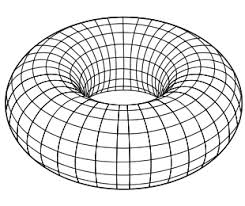
\includegraphics[height=1.5cm]{torus.jpg}}
	\logo{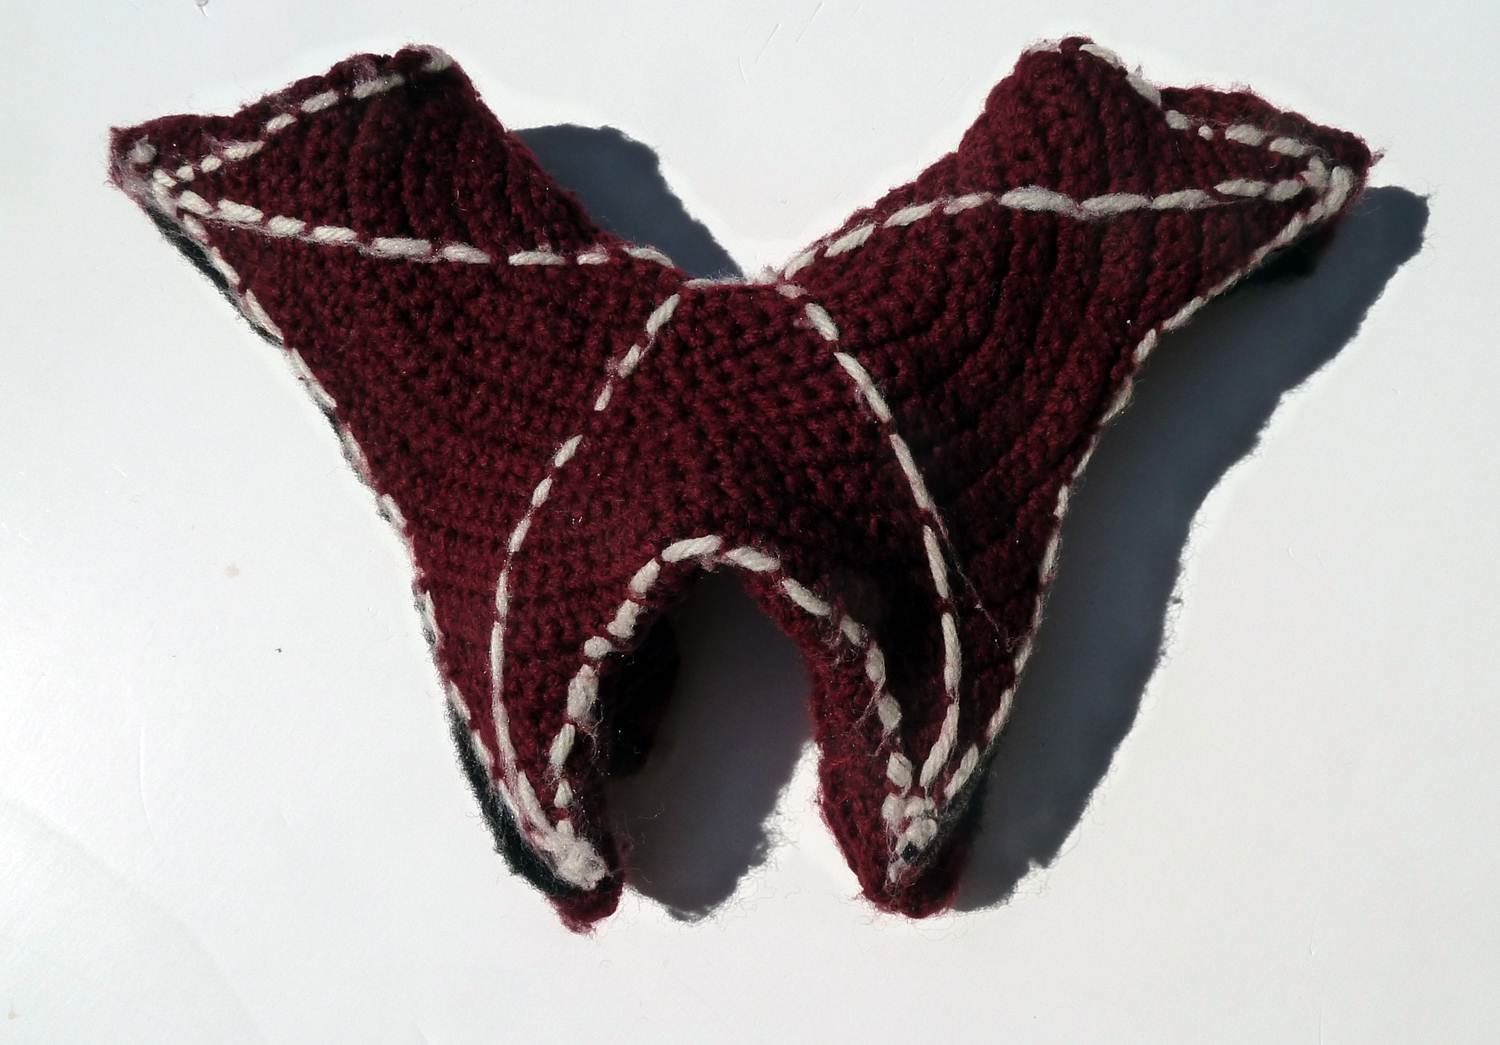
\includegraphics[height=1.5cm]{hyperbolicpants.jpg}}
	%torus, hyperbolic pants, double torus
\end{frame}

\begin{frame}
\frametitle{Gluings}
	\begin{itemize}
		\item \alert{Gluings} are when two edges or sides of a surface are ``connected'' and share the same set of points.
		% gluings for torus, mobius strip
	\end{itemize}
\end{frame}

\begin{frame}
\frametitle{Gluings}
	\begin{itemize}
		\item \alert{Gluings} are when two edges or sides of a surface are ``connected'' and share the same set of points.
		% gluings for torus, mobius strip
	\end{itemize}
\end{frame}

\section{Geometric 3-Manifolds} % ==========================================================================
% TITLE ------------------------------------------------
\begin{frame}
\frametitle{Geometric 3-Manifolds}
This is a text in first frame. This is a text in first frame. This is a text in first frame.
\end{frame}

\section{Cosmic Microwave Radiation} % ==========================================================================
% TITLE ------------------------------------------------
\begin{frame}
\frametitle{Cosmic Microwave Radiation}
This is a text in first frame. This is a text in first frame. This is a text in first frame.
\end{frame}

\section{The Shape of Space} % ==========================================================================
% TITLE ------------------------------------------------
\begin{frame}
\frametitle{The Shape of Space}
This is a text in first frame. This is a text in first frame. This is a text in first frame.
\end{frame}

% References ------------------------------------------------
 \begin{frame}[allowframebreaks]
  \frametitle{References}    
  \begin{thebibliography}{10}    
  \beamertemplatebookbibitems
  \bibitem{Autor1990}
    A.~Autor.
    \newblock {\em Introduction to Giving Presentations}.
    \newblock Klein-Verlag, 1990.
  \beamertemplatearticlebibitems
  \bibitem{Jemand2000}
    S.~Jemand.
    \newblock On this and that.
    \newblock {\em Journal of This and That}, 2(1):50--100, 2000.
  \end{thebibliography}
\end{frame}

\end{document}